\subsection{Гипербола}

{\bfseries \term{Гипербола}} --- геометрическое место точек евклидовой плоскости, абсолютное значение разности расстояний от которых до двух выделенных точек $F_1$ и $F_2$, называемых фокусами, постоянно.
\begin{equation}
	\big||F_1M|-|F_2M|\big| = \const.
\end{equation}

\begin{wrapfigure}[14]{r}{0.5\tw}
	\vspace{-1pc}
	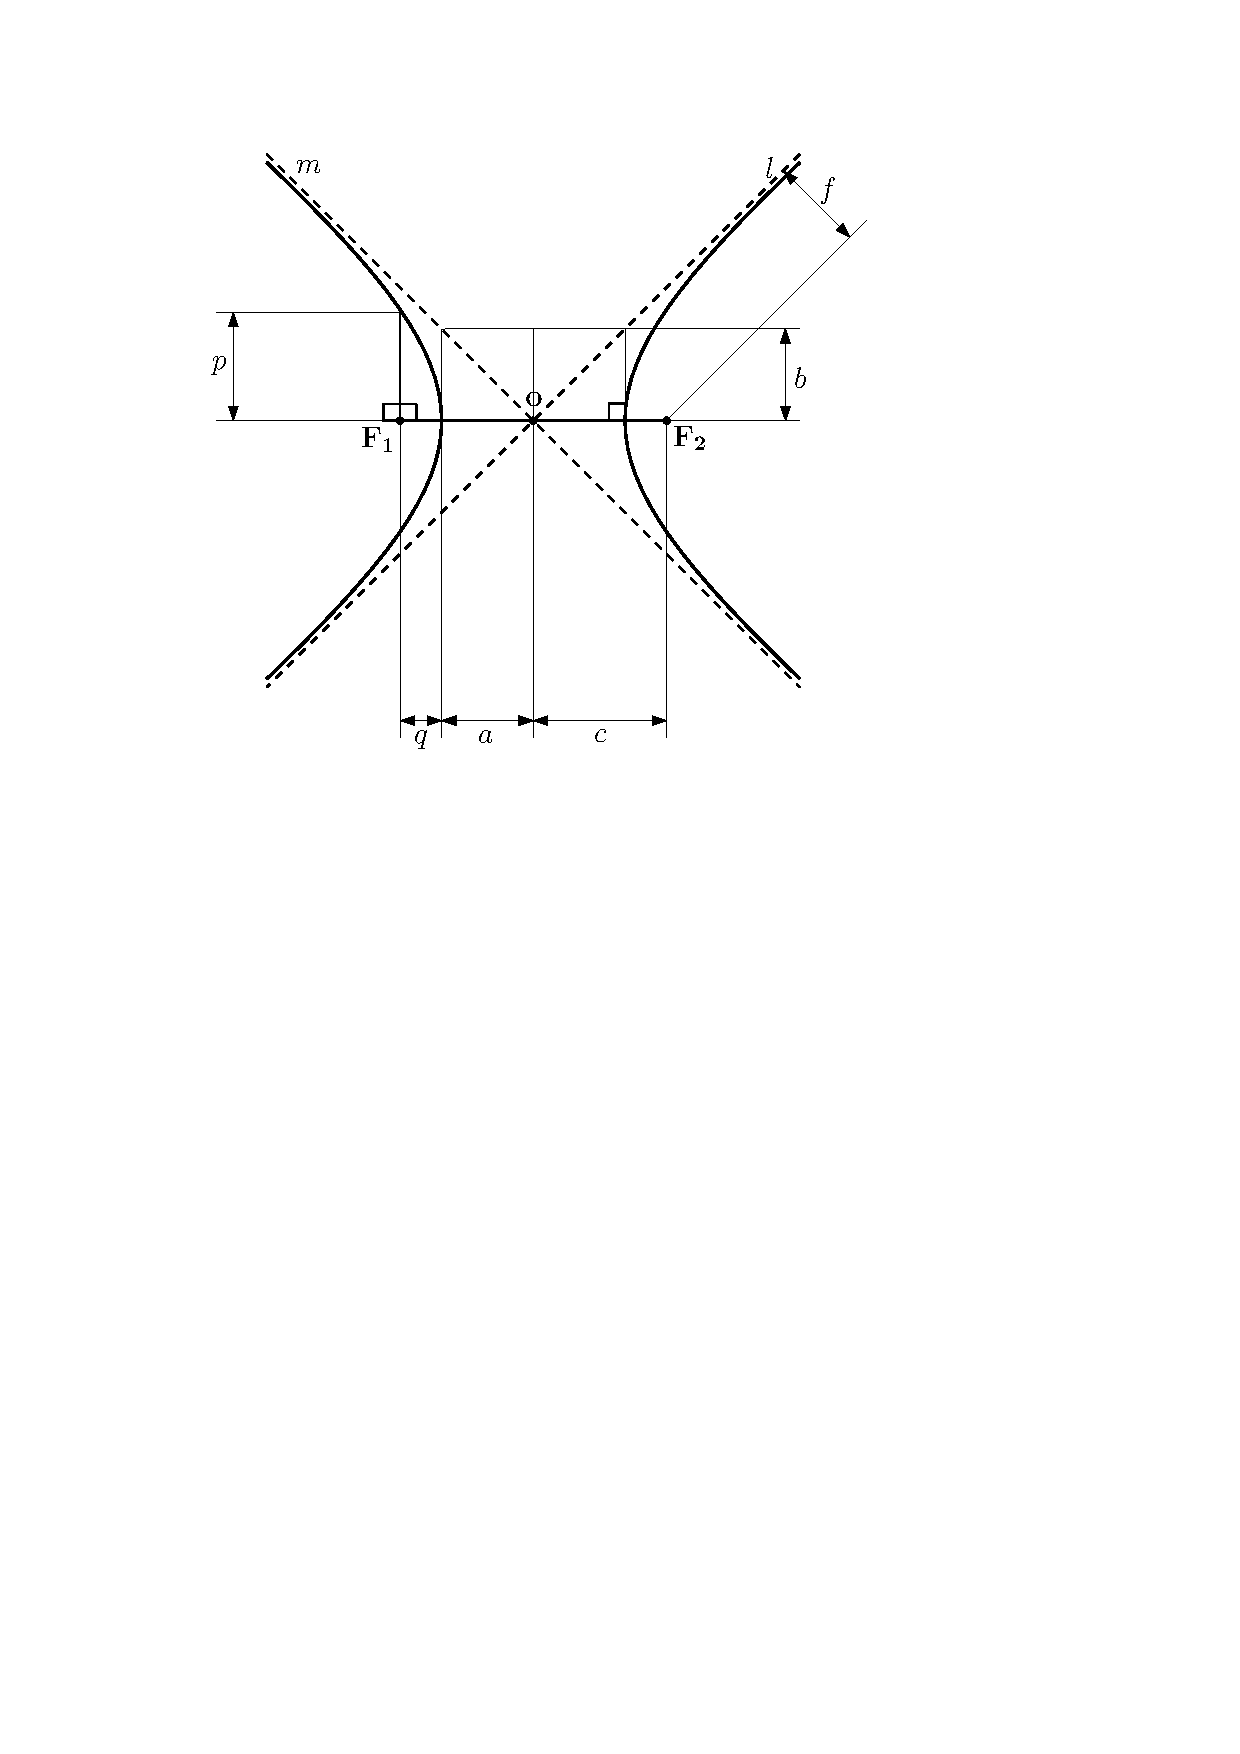
\includegraphics[width = 0.5\textwidth]{Hiperbola}
	\captionof{figure}{Гипербола \label{pic:the-pic}}
\end{wrapfigure}
Ближайшие друг к другу точки двух ветвей гиперболы называются \term{вершинами} гиперболы, а середина отрезка, соединяющего её фокусы~--- \term{центром}. \term[большая полуось]{Большая} или \term{действительная полуось}~($a$) гиперболы~--- расстояние от центра гиперболы до одной из вершин. \term{Фокальное расстояние}~($c$)~---  расстояние от центра гиперболы до одного из фокусов. \term[эксцентриситет]{Эксцентриситетом} гиперболы~($e$), как и  эллипса, является отношение фокального расстояния к большой полуоси, так как большая полуось гиперболы всегда меньше её фокального расстояния, эксцентриситет гиперболы больше единицы и согласно определению
\begin{equation}
	e=\frac{c}{a} > 1.
\end{equation}

\term{Перицентрическое расстояние} ($q$)~--- расстояние от фокуса до ближайшей вершины гиперболы. Очевидно, центр гиперболы, её фокусы и вершины лежат на одной прямой, являющейся ось симметрии гиперболы. Отсюда перицентрическое расстояние является разностью фокального расстояния и большой полуоси, то есть
\begin{equation}
	q = c - a = a (e - 1).
\end{equation}

Найдем модуль разности расстояний от вершины гиперболы до фокусов, тем самым найдем значение константы в определении гиперболы. 
\begin{equation*}
	\big||F_1 V| - |F_2 V|\big| = |q - (c + a)| = |a(e - 1) - a(e + 1)| = |-2a| = 2a.
\end{equation*}

Получим уравнение гиперболы в декартовых координатах. Пусть фокусы гиперболы находятся в точках $(\pm c, 0)$, а эксцентриситет равен $e$. Рассмотрим точку $A$ на гиперболе с координатами $(x,y)$. Подставим её координаты в определение гиперболы:
\begin{gather*}
	\big| |F_1 A| - |F_2 A| \big| = 2a,\\
	\left|\sqrt{(-c - x)^2 + y^2} - \sqrt{(c - x)^2 + y^2} \right| = 2a,\\
	(-c - x)^2 + y^2 + (c - x)^2 + y^2 - 2\sqrt{(-c - x)^2 + y^2}\sqrt{(c - x)^2 + y^2} = 4a^2,\\
	x^2 + c^2 + y^2  - \sqrt{(x^2 + c^2 + y^2 + 2cx ) ( x^2 + c^2 + y^2 - 2cx )} = 2a^2,\\
	x^2 + c^2 + y^2 - \sqrt{\big(x^2 + c^2 + y^2\big)^2 - 4 c^2 x^2} = 2a^2,\\
	\xi^2 - 4 c^2 x^2 = \xi^2 + 4a^4 - 4a^2\xi, \quad \xi \equiv x^2 + c^2 + y^2,\\
	a^4 - a^2 \xi + c^2x^2 = 0,\\
	1 - \frac{x^2}{a^2} - \frac{c^2}{a^2} - \frac{y^2}{a^2} + \frac{c^2}{a^2} \frac{x^2}{a^2} = 0,\\
	\frac{x^2}{a^2} (e^2 - 1) - \frac{y^2}{a^2} = e^2 - 1,\\
	\frac{x^2}{a^2} - \frac{y^2}{a^2(e^2 - 1)} = 1.
\end{gather*}
Вводя обозначение $b \equiv a \sqrt{e^2 - 1}$, получаем каноническое уравнение гиперболы:
\begin{equation}
	\frac{x^2}{a^2}-\frac{y^2}{b^2}=1.
\end{equation}

Найдем теперь асимптотическое поведение функции $y(x)$ при $x \rightarrow \pm \infty$, получив её из канонического уравнения гиперболы:
\begin{equation*}
	 y(x) = \pm b\sqrt{\frac{x^2}{a^2} - 1} =  \pm x \cdot \frac{b}{a}\sqrt{1 - \frac{a^2}{x^2}} \simeq \pm x \cdot \frac{b}{a}, \quad x \rightarrow \pm \infty.
\end{equation*}
Следовательно, ветви гиперболы асимптотически приближаются в прямым с коэффикиентом наклона $\pm b/a$, проходящим через центр гиперболы (начало координат). Эти прямые называются \term{асимптотами} гиперболы.

Заметим, что длина отрезка перпендикуляра, проведенного к оси гиперболы через одну из её вершин, от вершины до точки пересечения с асимптотой равна $b$, так как $|y(\pm a)| = b$. Данный отрезок является \term{мнимой полуосью} гиперболы. Важно отметить, что для длины мнимой полуоси выполняется равенство
\begin{equation*}
	b^2 = a^2 (e^2 - 1) = c^2 - a^2.
\end{equation*}

\term{Прицельный параметр}~($f$)~--- расстояние от фокуса до асимптоты гиперболы. Пусть угол наклона асимптоты равен $\alpha$, тогда известно, что $\tg \alpha = b/a$, отсюда
\begin{gather*}
	\tg^2 \alpha = \frac{\sin^2 \alpha}{\cos^2 \alpha} = \frac{\sin^2 \alpha}{1 - \sin^2 \alpha} = \frac{b^2}{a^2} = e^2 - 1,\\
	\sin \alpha =\sqrt{\frac{e^2 - 1}{1 + (e^2 - 1)}} = \frac{b}{c}.
\end{gather*}
Значит прицельный параметр
\begin{equation}
	f = c \sin \alpha = b.
\end{equation}

\term{Фокальный параметр}~($p$)~--- длина отрезка, перпендикулярного к действительной оси (оси симметрии), опущенного с гиперболы в точку её фокуса. Определяется формулой
\begin{equation}
	p= |y(c)| = b\sqrt{\frac{c^2}{a^2} - 1} = b \sqrt{e^2 - 1} = \frac{b^2}{a}.
\end{equation}

Найдем уравнение гиперболы в полярных координатах. Для сделаем замены $x = r \cos \varphi$ и $y = r \sin \varphi$ в каноническом уравнении гиперболы:
\begin{gather*}
	\frac{r^2 \cos^2 \varphi}{a^2} - \frac{r^2 \sin^2 \varphi}{b^2} = 1,\\
	r^2 ( b^2 \cos^2 \varphi - a^2 \sin^2 \varphi) = a^2 b^2,\\
	r^2 \big( (a^2 + b^2) \cos^2 \varphi - a^2 \big) = a^2 b^2,\\
%	r = \pm\frac{ab}{\sqrt{c^2 \cos^2 \varphi - a^2}},\\
	r = \pm\frac{b}{\sqrt{e^2 \cos^2 \varphi - 1}}.
\end{gather*}

Проделаем тоже самое, только полюс полярных координат поместим в фокус с координатами $(c,0)$. Для этого нужно сделать замену $x' \hookrightarrow x - c$, обратно, $x \hookrightarrow x' + c$. Остаётся перейти к полярным координатам: $x' = r \cos \varphi$, $y = r \sin \varphi$, в каноническом уравнении гиперболы в декартовых координатах.
\begin{gather*}
	\frac{(r \cos \varphi + c)^2}{a^2} - \frac{r^2 \sin^2 \varphi}{b^2} = 1,\\
	 b^2 r^2 \cos^2 \varphi + 2 b^2 r c \cos \varphi + b^2 c^2 - a^2 r^2 \sin^2 \varphi = a^2 b^2,\\
	 (a^2 + b^2) r^2 \cos^2 \varphi + 2 b^2 r c \cos \varphi + b^2 c^2 - a^2 r^2 = a^2 b^2,\\
	(rc\cos \varphi + b^2)^2 + b^2(c^2 - b^2) - a^2 r^2 = a^2 b^2,\\
	(rc\cos \varphi + b^2)^2 = a^2 r^2,\\
	rc\cos \varphi + b^2 = -a r,\quad\text{т. к.}~r(0) = -q,\\
	r = \frac{b^2}{-a - c \cos \varphi} = - \frac{p}{1 + e \cos \varphi}.
\end{gather*}
Можно считать, что перицентр гиперболы достигается при $\varphi = 0$, то же самое, что повернуть ось отсчёта углов на угол $\pi$, тогда в знаменателе будет знак <<$-$>>. Окончательно, каноническое уравнение гиперболы в полярных координатах принимает вид:
\begin{equation}
	r = -\frac{p}{1 \pm e \cos \varphi}.
\end{equation}

Также, как и остальные конические сечения, гипербола имеет своё \imp{оптическое свойство}: свет от источника, находящегося в одном из фокусов гиперболы, отражается ветвями гиперболы таким образом, что продолжения отраженных лучей пересекаются во втором фокусе.

Для доказательства оптического свойства гиперболы положим, что фокусы имеют координаты $(\pm c, 0)$, где $c$~--- фокальное расстояние гиперболы, а произвольная точка гиперболы имеет координаты $(x, y)$ принадлежит гиперболе. Будем для удобства считать, что $y > 0$, случай $y < 0$ рассматривается аналогично. Тогда каноническое уравнение гиперболы можно представить в виде функции $y(x)$. При этом направляющий вектор $\vec t$ касательной к гиперболе в точке $(x, y)$, очевидно, можно представить, как
\begin{equation*}
	\vec t = 
	\begin{pmatrix}
		1\\
		y'(x)
	\end{pmatrix} = 
	\begin{pmatrix}
		1\\
		\dfrac{bx}{a \sqrt{x^2 - a^2}}
	\end{pmatrix}.
\end{equation*}

Пусть источник находится в фокусе с координатами $(c, 0)$, тогда направляющий вектор луча, испущенного в точку $(x, y)$ равен $\vec r = (x - c, y)$, а луча отраженного по предположению $\vec r' = (x + c, y)$. При этом из определения гиперболы следует, что $|\vec r'| = |r| + 2a$, чем мы воспользуемся ниже. 

Остается показаться, что углы $\widehat{\vec r \vec t}$ и $\widehat{\vec t \vec r'}$. Для этого достаточно обосновать равенство их косинусов, которые можно выразить с помощью скалярного произведения:
\begin{gather*}
	\frac{ \scalar{r}{t}}{|\vec r| | \vec t |} = \frac{ \scalar{r'}{t}}{|\vec r'| | \vec t |},\\
	\frac{ x - c + y'(x)y(x)}{|r|} = \frac{x + c + y'(x) y(x)}{|r| + 2a},\\
	\frac{ x - c + \dfrac{bx}{a \sqrt{x^2-a^2}} \cdot \dfrac{b\sqrt{x^2 - a^2}}{a}}{\sqrt{(x - c)^2 + y^2}} = \frac{ x + c + \dfrac{bx}{a \sqrt{x^2-a^2}} \cdot \dfrac{b\sqrt{x^2 - a^2}}{a}}{\sqrt{(x - c)^2 + y^2} + 2a},\\
	\frac{ x - c + \dfrac{b^2 x }{a^2}}{\sqrt{(x - c)^2 + y^2}} = \frac{ x + c + \dfrac{b^2 x }{a^2}}{\sqrt{(x - c)^2 + y^2} + 2a},\\
	2ax - 2c\sqrt{(x - c )^2 + y^2} - 2ac + \frac{b^2 x}{a^2} \cdot 2a = 0,\\
	\left( ax - ac + \frac{b^2 x}{a} \right)^2 = c^2 \left( (x-c)^2 + \frac{b^2 (x^2 - a^2)}{a^2} \right).
%	a^2 x^2 + a^2 c^2 + \frac{b^4 x^2}{a^2} - 2 a^2 c x + 2 b^2 x^2 - 2 b^2 c x = c^2 \big( (x-c)^2 + y^2 \big)\\
%	c^2 x^2  + b^2 x^2 + a^2 c^2 + \frac{b^4 x^2}{a^2} - 2 c^3 x = c^2 \left( x^2 - 2xc + c^2 + \frac{b^2 x^2}{a^2} - b^2 \right),\\
%	b^2 x^2 + a^2 c^2 + \frac{b^4 x^2}{a^2} = c^4 + \frac{b^2 c^2 x^2}{a^2} - b^2 c^2,\\
\end{gather*}
Приводя подобные слагаемые с учетом равенства $c^2 = a^2 + b^2$ несложно показать тождественность полученного равенства.

